\chapter{Politeness}\label{chp-polite}
\section{Overview}
Politeness is suite of policies and de-facto standards. Essentially, they exist to prevent a crawler annoying the webmaster of a site its crawling. This might happen for a number of reasons:
\begin{itemize}
\item{The crawler is accessing parts of a website the webmaster would prefer it didn't.}
\item{The crawler is accessing to website at too high a speed.}
\end{itemize}
Annoying a webmaster is counter-productive, because they may prevent the crawler from accessing their website in the future. This means that the content cannot be crawled and hence the index cannot deliver results from those pages.

\section{Robots Exclusion}
\subsection{Background}
There are two forms of Robots Exclusion protocol that crawlers must obey. Firstly, the robots.txt\cite{site4} file allows the webmaster of a site to place control over what pages a web crawler will fetch. Secondly, the meta-robots directive\cite{site5} in the HTML source of a page will provide essentially the same control.
\subsection{robots.txt}
The robots.txt\cite{site4} protocol is a file which a crawler must first fetch from each host before it crawls the host. Although its presence is optional, the crawler must fetch http://hostname/robots.txt and parse the file to recognise the rules it contains. Below can be found an example of a robots.txt file.
\renewcommand{\baselinestretch}{1.0}
\begin{verbatim}
#robots.txt file from http://www.dcs.gla.ac.uk/
User-agent: *
Disallow: /cgi-bin/
Disallow: /people/
\end{verbatim}\\
\renewcommand{\baselinestretch}{1.5}
Each robots.txt file has list of rules which specifies which directories may not be crawled by any crawler. It can also specify, using the User-agent directive, any directories exclusions specific to a particular crawler. In the example, no crawlers are permitted to fetch any URLs starting http://www.dcs.gla.ac.uk/cgi-bin/ or http://www.dcs.gla.ac.uk/people/.\\
\ \\
When any crawler of Labrador finds a host it has not visited before, it checks its local robots.txt cache to see if a copy of the robots.txt file has been downloaded. If this is not the case, then the dispatcher's robots.txt cache is checked as well, before downloading the file itself. When any crawler downloads a robots.txt file, it will send a copy of the file to the dispatcher to be added to the global cache. By default, Labrador caches robots.txt files for 25 days, although this can be altered by the RobotsTxtExpiry in the configuration file.
\subsection{Meta-Robots}\label{sect-metarobots}
The Meta-Robots\cite{site5} specifies an alternative to the robots.txt standard, which is specified in a meta tag in the HTML of the page. Traditionally meta tags have been used to specify other meta data for a search engine to use during the indexing phase, such as document keywords or a description, but soon after the robots.txt standard was introduced, the web authors wanted more fine-grained control than the robots.txt file provided. The meta-robots standard allowed web authors to specify whether a crawler should index a page without having to change the robots.txt file. This was particularly useful when the author of the document did not have control over the robots.txt file of the server they were using - for example a shared hosting environment.
\indent \begin{verbatim}<meta name="robots" content="noindex">\end{verbatim}\\
Above is an example meta-robots directive that specifies that a crawler may not index that page. The values supported by the meta-robots directive is shown in Table \ref{tbl-metarobots}.
\renewcommand{\baselinestretch}{1.0}
\begin{table}
\begin{center}
\begin{tabular}{|l|l|}
\hline
\bf{Directive} & \bf{Description} \\
\hline
none & A crawler may not follow links from this page, nor index the contents.\\
\hline
noindex & A crawler may not index the contents of this page \\
\hline
nofollow & A crawler may not follow links on this page \\
\hline
all & A crawler may index this page and follow its links \\
\hline
\end{tabular}
\caption{Meta-Robots directives}\label{tbl-metarobots}
\end{center}
\end{table}
\renewcommand{\baselinestretch}{1.5}

\section{Host Delay}
\subsection{What is Host Delay?}
Host Delay (or per-host delay) relates to the directive in Labrador's configuration file that specifies the delay in seconds between each request to a given host. It is part of the politeness protocols, because by crawling a host too fast, the crawler is likely to annoy the server's webmaster:
\begin{itemize}
\item{Uses bandwidth which costs the webmaster's organistion.}
\item{The crawl may be mistaken for a Denial of Service attempt.}
\item{Otherwise interfere with the day-to-day running of the website. For instance, the site may become slow because of the crawler, thus detracting potential customers.}
\end{itemize}

\subsection{Why is Host Delay a problem for a crawler?}
There are two essential problems with Host Delay:
\begin{itemize}
\item{An efficient implementation that correctly queues URLs, such that the delay is respected, is complex to develop.}
\item{The amount of time that it adds to a crawl, compared to crawling the same site with no delay.}
\end{itemize}


\subsection{Host Delay queuing implementations}\label{sect-hostdelayimpls}
I attempted several queuing implementations before I found a solution which was both correct and efficient.
\subsubsection{Re-queuing of URLs}
My first attempt at implementing a per-host delay system involved pushing URLs that were deemed too early back into the queue, at a place thought to be approximately correct. I tried this using two different heuristics:
\begin{itemize}
\item{Using the current URLs/sec rate to approximate a position in the queue.}
\item{Using the current URLs/sec rate and the position in the queue of the most recent URL seen for that host.}
\end{itemize}
Both these heuristics were found to be inefficient. This was primarily due to locality in links found on HTML pages (most sites link to pages in their own site\cite{ref17}), which meant that queues tended to consist of groups of URLs for the same host. The algorithm would push each URL back as far as it thought it needed to be in the queue to cause host delay. However, the crawler would end up working through all URLs at the head of the queue, without finding a URL that was ready to be fetched.

\subsubsection{Queues for each second of delay and queue promotion}
Another implementation I attempted was to use a set of arrays, each array representing x-many seconds of delay. URLs were sorted onto an appropriate delay array, based on how much the previous URL for that host was delayed and when that event ocurred. Once every second, each queue was promoted - i.e. queue 4 became queue 3, queue 5 became queue 4 and so on. This prevents URLs from being fetched before they are ready.\\
\ \\
\begin{figure}[h]
  \centerline{
    \epsfig{file=./images/slicedqueue.eps, scale=0.7}
  }
  \caption{Sliced Queue}
  \label{fig-slicedqueue}
\end{figure}
\ \\
This implementation was found to be inefficient, as when crawling on an institution scale, the crawler was often delaying URLs by tens of thousands of seconds of delay and hence requiring tens of thousands of separate queues. At this size, the overhead of promoting all the queues once each second became critical. This problem could have been eliminated using a renumbering of the queues during promotion instead of moving data between queues. However, this was deemed less favourable than an attempt at using DelayLines, as described below.

\subsubsection{DelayLine of URLs}
A DelayLine\cite{site1} is a sorted array where each element has a `not before time' tagged onto it. De-queuing is a constant-time operation, while inserts are O(nlog n). At first I tried using a DelayLine for all URLs in the system, delaying each URL based on the amount of delay the previous URLs has had (or time since last fetch if no other requests for that host are currently queued). However, again as the delayline for single crawler became nearer 40,000 URLs for a medium size crawl, the insert operation became prohibitively expensive. I could have improved the insert operation to O(log n) time, but then deemed that this would not provide the level of performance required.

\subsubsection{DelayLine of Hostnames and queues for each hostname}
My final implementation of a per-host delay data structure was using a separate queue for each host of the crawler and a DelayLine, as described above, to provide the delaying of each host. This can be seen in Figure \ref{fig-delaylinehosts}. The URLAlloc Delay module dequeues a hostname that is ready for every request by the crawler Manager. Being ready means that the time since the last fetch from that host exceeds the Host Delay setting. This dequeued hostname tells the Delay module from which queue it should next dequeue a URL. If the DelayLine has no hosts that are ready to fetch, then the crawler will determine how long it has to wait and if no URLs are available from the dispatcher, then the crawler will sleep until there are some ready. Due to the fact that there are few hosts active for a crawler at any one time, this implementation is as efficient as desired and correct, in as much as it prevents URL fetches before they are ready.

\begin{figure}[h]
  \centerline{
    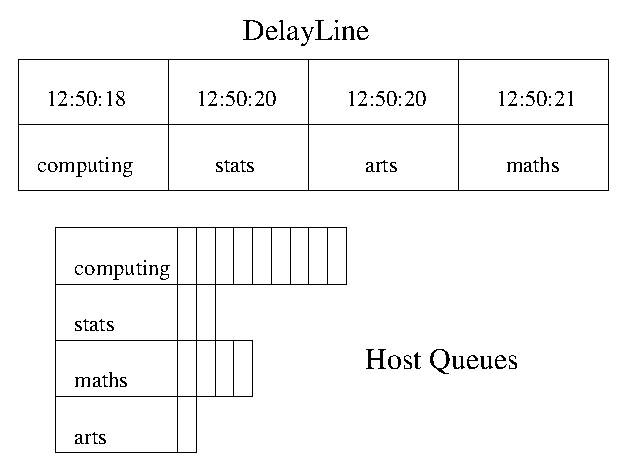
\epsfig{file=./images/delayline_hosts.eps, scale=1.0}
  }
  \caption{Delay internals: Host queues and a DelayLine of hostnames.}
  \label{fig-delaylinehosts}
\end{figure}

\subsubsection{Approximate permutations of URLs into chunks}
Many crawlers use hashing functions, e.g. $k$-way unshuffle permutations\cite{ref1}, to group URLs into chunks, which have enough URLs of different hosts in each chunk to ensure that the crawler will be kept busy without fetching from any one host too often. This method has the advantage that no sorting needs to be done at insert time, and overheads are minimised as URLs are chunked. I believe that each chunk of URLs would still have to be marked with a time that it cannot be fetched before, because towards the end of a crawl when the crawler were running out of hosts, they might run through the chunks too quickly, resulting in insufficitently delayed requests.
\subsection{Host Delay time issue}
Once a few crawls have been performed by a crawler that correctly implements a Host Delay functionality, it becomes apparent that the rate at which URLs can be fetched could be severly hampered. Adding more crawlers does not improve the URL rate. Quite simply, the crawlers do not have enough work to keep them `entertained'. This means that at a given time during a crawl, some crawlers may be asleep, as they have recently fetched from all their allocated hosts. They are not permitted to fetch from any host until the Host Delay has expired for that host. They may try asking the dispatcher if it has any more URLs it can give it, but often this is not sufficient to keep them busy.\\
\ \\
In fact, the time taken to completely crawl a domain ($T$), can be expressed as:
\ \\
\indent $T \geq HostDelay \times (size\ of\ largest\ site\ in\ domain)$
\ \\
Note that this is irrespective of the number of crawlers, or of the size of the domain.
Due to this, during a typical crawl the URL rate diminishes towards the end of the crawl, as more and more sites have had all their discovered pages retrieved.\\
\ \\
Empirically, let's examine the domain gla.ac.uk:

There are 200 sites with less than 100 pages and only 4 with greater than 30,000 pages, ignoring manually blacklisted spider traps. With a Host Delay of 3 seconds, any crawl of of gla.ac.uk can be no shorter than 30,000 * 3 seconds, i.e. 25 hours. Note that increasing the number of crawlers may increase the fetch rate when the crawlers are backlogged, but will have no effect on the minimum crawl time. However, normal crawls take longer than the minumum, as explained in Section \ref{sect-discovery}.
\ \\
Interestingly, the distribution of host sizes versus frequency follows a power-law distribution, as can be seen in \ref{fig-hostsizedistribution}. This graph was drawn using host sizes found during crawls of the universities of Glasgow, Strathclyde, Paisley and Glasgow Caledonian. A larger crawl may produce a clearer distribution, as documented by Huberman and Adamic (1999)\cite{ref15} who used information from crawls by Alexa and Infoseek.

\begin{figure}[h]
  \centerline{
    \epsfig{file=./images/log_e.ps, height=5in, angle=-90}
  }
  \caption{Distribution of host size versus frequency}
  \label{fig-hostsizedistribution}
\end{figure}

\subsection{Discovery period}\label{sect-discovery}
In the formula above, the reader should note that I have stated $\geq $ and not a direct equality. This is due to what I have determined to be the discovery period. This essentially comes in two varieties, host discovery and URL discovery.\\
\ \\
For example, for a crawl of the gla.ac.uk domain seeded with just the University homepage, http://www.gla.ac.uk/, where every page in the domain is eventually reachable from the homepage, the URL rate at first will be poor, but will increase as more hosts are discovered. This means that the crawlers spend less time idle waiting to be allowed to access their allocated hosts again.\\
\ \\
Similarly, a site may only be half crawled by a crawler, as the site may happen to have its links partitioned into n-partite sections. The next section will only be discovered when crawling another separate site. If this is a big site then valuable time will have been lost in the gap between one partition of the site being finished and another one being discovered. This is the problem of URL discovery.\\
\ \\
Discovery period can be minimised when doing subsequent crawls of a domain by seeding the crawler with all URLs fetched during the previous crawl. This means that the host and URL discovery period will be mostly eliminated, although new hosts and URLs since the previous crawl still have to be discovered. This immensly speeds up the initial URL fetch rate and is the most effective way of speeding up a crawl, apart from shortening the host delay. Most commercial search engines seed their crawlers with URLs of the previous crawl to minimise the discovery period effect (Google prioritises the URLs by PageRank as well\cite{ref5}).
